\documentclass[referee,sn-basic]{sn-jnl}

%%%% Standard Packages
%%<additional latex packages if required can be included here>

\usepackage{graphicx}%
\usepackage{multirow}%
\usepackage{amsmath,amssymb,amsfonts}%
\usepackage{amsthm}%
\usepackage{mathrsfs}%
\usepackage[title]{appendix}%
\usepackage{xcolor}%
\usepackage{textcomp}%
\usepackage{manyfoot}%
\usepackage{booktabs}%
\usepackage{algorithm}%
\usepackage{algorithmicx}%
\usepackage{algpseudocode}%
\usepackage{listings}%
\usepackage{hyphenat}
\usepackage[T1]{fontenc}

\theoremstyle{thmstyleone}%
\newtheorem{theorem}{Theorem}%  meant for continuous numbers
\usepackage[portuguese]{babel}
\raggedbottom
%%\unnumbered% uncomment this for unnumbered level heads



\begin{document}

\title[Article Title]{Ética aplicada à Evolução Tecnológica}



\abstract{\hspace{0.7cm}  É muito fácil notar os benefícios que a tecnologia traz no dia a dia das pessoas. Fazer compras e marcar consultas ‘online’, criptomoedas e investimentos são mais acessíveis, e até mesmo casais inférteis que conseguem gerar uma criança com ajuda da fertilização in vitro. Mas assim como todas as coisas, também temos um lado negativo: as implicações éticas dessas tecnologias. Tópicos como este necessitam do toque humano com a sua subjetividade e emoção, para podermos aprimorar a nossa aliada, a tecnologia, à nossa vontade.  Entendemos que diferentes pontos de vista podem levar a diferentes conclusões do que é certo ou errado em alguns momentos, mas o maior objetivo deste artigo é trazer conhecimento e começar discussões sobre a importância deste tópico, que parece ser esquecido tão regularmente. O foco é levar o leitor a exercitar o seu senso crítico, para que futuramente saiba identificar casos de má ética do uso das tecnologias e proteger-se de tal situação.}

\keywords{Ética em IA, Progresso tecnológico e moralidade, Ética Digital, Inovação responsável}

\maketitle

\newpage

\section{Introdução}\label{sec1}

\hspace{0.7cm}A tecnologia tem sido um dos temas dominantes na atualidade. No entanto, um problema que ainda não recebeu a devida atenção por parte de especialistas e usuários de tecnologia é a questão ética subjacente a ela. Nesse sentido, tomamos a iniciativa de escrever este artigo com o objetivo de explorar esse tema e levá-lo a um público mais amplo. Apresentamos neste artigo algumas fontes que consideramos interessantes e discutimos tanto os resultados éticos de tecnologias atuais quanto teóricas.\par 
Alguns podem argumentar que a ética é um assunto completamente subjetivo. No entanto, consideramos que a ética possui uma lógica própria, assim como a matemática, por exemplo. O que pode torná-la subjetiva é a maneira como é abordada ou avaliada sob diferentes conjuntos de regras (como uma visão utilitarista do que é certo ou errado). Portanto, reconhecemos que é possível que o leitor não concorde com nosso ponto de vista. Nosso objetivo não é fazer com que o leitor aceite completamente o que estamos dizendo ou tentar definir princípios éticos de alguma forma, mas sim incentivá-lo a questionar-se e refletir sobre este importante tópico.


\section{Debates éticos da IA}

\hspace{0.7cm}O avanço tecnológico atual nos leva ao desenvolvimento da Inteligência Artificial, mas quão éticas podem ser as IA? Quem tem a responsabilidade de respeitar a ética? A IA ou seu criador/dono? Perguntas como essas vêm de uma pergunta principal que precisa ser respondida primeiro: "Se o software se parece com um cérebro e age como um cérebro, vamos tratá-lo como tal?" \cite{morber2015software}\par

Primeiro, é importante questionar se a Inteligência Artificial (IA) realmente representa um sistema intelectual. Alguns especialistas argumentam que o que rotulamos como IA ainda é principalmente um sistema de Machine Learning \cite{schmelzer2019}. Mas o que constitui a inteligência? De acordo com Jean Khalfa, inteligência são "as ferramentas da mente que nos dão acesso à experiência acumulada da humanidade, permitindo-nos raciocinar, testar nossas ideias e planejar para o futuro" \cite{Khalfa1994-KHAWII-2}. No entanto, os sistemas atuais são incapazes de realizar essas tarefas. A IA até poderia simular a inteligência humana, mas isso não é um requisito \cite{mccarthy2007artificial}. Se algo não é como nós, como podemos tratá-lo como se fosse? A resposta é clara: não podemos. Se esse é o caso, como podemos responsabilizar a IA pela ética? Também não podemos fazer isso; a responsabilidade recai sobre seu criador/dono.


\subsection{Ética no Método de Funcionamento da IA}
\hspace{0.7cm}Benj Edwards, em seu artigo sobre o Microsoft Designer e o DALL-E 2, levanta preocupações importantes sobre o uso de fotos online por ferramentas de IA para criar novas imagens sem o consentimento dos criadores ou detentores dos direitos autorais \cite{edwards2022microsoft}.\par

A Microsoft selecionou o DALL-E 2, uma IA desenvolvida pela OpenAI, como a base para sua nova ferramenta, o Microsoft Designer. Esta IA gera imagens a partir de descrições textuais fornecidas pelos usuários, utilizando fotos disponíveis online como fonte. Edwards argumenta que este método de funcionamento é antiético, pois viola os direitos dos criadores das imagens originais, que não consentiram com o uso de suas obras para tais propósitos.\par

\subsubsection{Argumentos a Favor do Uso de Imagens Online por IA}
\hspace{0.7cm}Os defensores do uso de imagens online por IA argumentam que a internet é uma plataforma aberta, onde a disseminação de imagens é frequentemente implícita pelo ato de publicar. A utilização dessas imagens como inspiração para criar novas obras, de acordo com essa visão, não difere fundamentalmente da prática histórica de artistas que se inspiram em elementos do mundo ao seu redor. Nesse contexto, a IA age de forma semelhante a um artista humano, processando e reinterpretando imagens para gerar novas criações.\par

Além disso, a capacidade de uma IA como o DALL-E 2 de gerar imagens a partir de descrições textuais pode ser vista como uma inovação tecnológica que amplia as possibilidades criativas e democratiza o acesso à arte e ao design. Ferramentas como o Microsoft Designer podem permitir que pessoas sem habilidades artísticas tradicionais criem visuais impressionantes, fomentando a criatividade e a expressão pessoal. Outro argumento a favor é que a reutilização de imagens online pode ser considerada um uso justo, especialmente se as novas obras criadas pela IA forem transformativas, ou seja, se acrescentarem novos significados, propósitos ou elementos às imagens originais. Em muitos sistemas jurídicos, o uso justo permite certos usos limitados de materiais protegidos por direitos autorais sem permissão, especialmente para fins como crítica, comentário, reportagem, ensino e pesquisa.\par

\subsubsection{Argumentos Contra o Uso de Imagens Online por IA}
\hspace{0.7cm}Por outro lado, os críticos, incluindo Benj Edwards, argumentam que o uso de imagens online por IA sem o consentimento dos criadores ou dos detentores dos direitos autorais é antiético e pode constituir uma violação dos direitos de propriedade intelectual. O direito autoral existe para proteger os interesses dos criadores, garantindo que eles possam controlar como suas obras são utilizadas e receber compensação justa pelo seu trabalho. Utilizar fotos online sem permissão para criar novas imagens pode ser comparado à apropriação indevida de propriedade intelectual. Essa prática desrespeita o trabalho e o esforço dos criadores originais, privando-os do reconhecimento e da remuneração que merecem. Além disso, a falta de atribuição adequada pode levar a um ambiente em que os criadores são desvalorizados e desencorajados a compartilhar suas obras. Outro ponto crucial é que muitos criadores publicam suas obras online com a expectativa de que seus direitos serão respeitados. A presunção de que qualquer imagem disponível na internet está livre para uso ignora a complexidade dos direitos autorais e as expectativas dos criadores. Esse comportamento pode criar um precedente perigoso, onde a proteção das obras criativas é enfraquecida, e o valor da propriedade intelectual é reduzido.\par

A preservação dos direitos autorais é fundamental para manter um ecossistema criativo saudável. Se as imagens estão disponíveis online, isso não implica automaticamente que elas são de domínio público ou que podem ser usadas livremente para qualquer propósito. Muitos criadores disponibilizam suas obras online para compartilhar seu trabalho, mas isso não deve ser interpretado como um consentimento implícito para usos não autorizados. Em conclusão, a responsabilidade ética no uso de IA deve incluir um compromisso claro com o respeito aos direitos autorais. As ferramentas de IA, como o DALL-E 2, devem ser projetadas para operar dentro dos limites legais e éticos estabelecidos, assegurando que os criadores sejam reconhecidos e que suas obras não sejam exploradas sem consentimento. Assim, preservamos o valor das criações individuais e incentivamos um ambiente de respeito e inovação.\par


\subsection{Ética na Evolução Tecnológica}
\hspace{0.7cm}Olhando para outros debates éticos, vamos falar sobre o artigo escrito por Vincent Muller, onde ele menciona diferentes tópicos de grande implicação ética \cite{sep-ethics-ai}, porém daremos ênfase para os que podem ser melhor aplicados na sociedade atual: Privacidade e Vigilância, Interação Humano-Robô (em parte), Automação e Emprego.


\subsubsection{Privacidade e Vigilância}
\hspace{0.7cm}Discutir Privacidade e Vigilância é crucial, já que a maior parte das pessoas ignoram as políticas e acordos de privacidade das aplicações e sites, levando a não saberem com o que estão a concordar. No entanto, é inegável que todos dependemos de dinheiro em certa medida, então como empresas como Meta ou TikTok se sustentam enquanto oferecem aplicativos gratuitos?\par

 Mullet aborda este tópico com uma declaração contundente: "O rastro de dados que deixamos para trás é como nossos serviços 'gratuitos' são pagos" \cite{sep-ethics-ai}. Esses dados muitas vezes são usados para nos manipular, influenciando sutilmente nossas escolhas. Por exemplo, é possível reparar em como anúncios de produtos que pesquisámos anteriormente online aparecem de repente enquanto navegamos na internet. É um acontecimento comum, mas muitos de nós simplesmente ignoramos sem considerar como os nossos dados estão a ser usados para personalizar esses anúncios.\par

Surge a pergunta: "O que acontecerá com a sociedade, a política e a vida quotidiana quando algoritmos não conscientes, mas altamente inteligentes, nos entenderem melhor do que nós entendemos a nós mesmos?" \cite{sep-ethics-ai}. É uma pergunta que nos faz refletir e com implicações perturbadoras. Só podemos esperar que as autoridades legais estejam preparadas para abordar e prevenir tal uso indevido de dados pessoais, protegendo nossa privacidade e integridade societal.



\subsubsection{Interação Humano-Robô}
\hspace{0.7cm}Outro debate ético referido por Muller é a Interação Humano-Robô \cite{sep-ethics-ai}, onde fala sobre tópicos com grande peso ético. Como por exemplo, a possibilidade de os humanos serem manipulados por robôs IA. Segundo o autor, os humanos têm uma tendência a "atribuir propriedades mentais a objetos e simpatizar com eles, especialmente quando a aparência externa desses objetos é semelhante à dos seres vivos" \cite{sep-ethics-ai}, mas tendo em conta a facilidade de adaptação da humanidade, por mais provável que seja esta situação, eventualmente esta manipulação deixaria de ter poder, no nosso ponto de vista.\par

Outro tópico discutido nesta secção são os robôs de cuidado, que poderiam diminuir o fator de “erro humano”, mas o cuidado não é apenas uma necessidade, mas sim um tipo de afeto entre humanos, algo que os robôs não oferecem da mesma forma. Ao substituirmos isso por máquinas, perdemos cada vez mais da nossa humanidade.


\subsubsection{Influência da evolução tecnológica no emprego}
\hspace{0.7cm}Já que mencionamos os possíveis usos das máquinas, podemos mencionar também a automação e o emprego. Muller apontou que no passado, os robôs físicos ajudaram a humanidade a chegar num nível tão avançado \cite{sep-ethics-ai}. A verdade é que os robôs também ajudam os humanos a encontrar soluções para problemas acima da capacidade humana, como o cancro e a Covid-19, mas também é mencionado um novo tipo de robôs, que não vão substituir os nossos empregos físicos, mas também os intelectuais.\par
\begin{figure}[h]
    \centering
    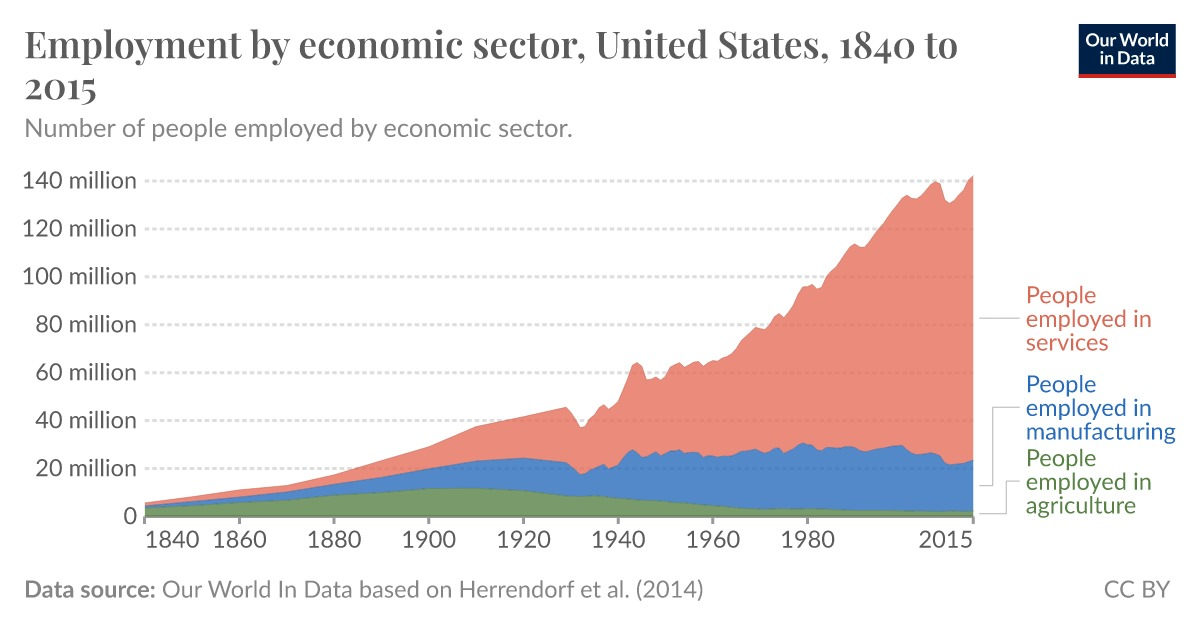
\includegraphics[width=1.\textwidth]{employing.jpg}
    \caption{Emprego por setor económico, EUA. 1840 até 2015.}
     \label{fig:employ}
\end{figure}

Devemos nos preocupar com tal declaração pois com a chegada das máquinas na Revolução Industrial, tivemos uma grande crise já que a maior parte da população estava a trabalhar no setor primário e secundário. Com o tempo houve maior necessidade de obter um maior grau académico, já que os trabalhos físicos foram automatizados (Figura \ref{fig:employ}).

\hspace{0.7cm}Se a chegada dos robôs intelectuais se concretizar, as máquinas substituiriam o esforço físico e intelectual dos seres humanos. Sendo assim, qual seria o nosso papel no mundo? Muller traz outra questão em relação a isso: "o desenvolvimento da IA é ambientalmente sustentável"? \cite{sep-ethics-ai}. O consumo requerido por essas máquinas é muito superior ao simples esforço humano, além disso, "sistemas de IA produzem resíduos que são muito difíceis de reciclar" \cite{sep-ethics-ai}. Estas perguntas tão simples nos fazem refletir que os impactos ambientais também são eticamente relevantes, pois se criamos máquinas que destroem os recursos do nosso planeta, onde viveremos.


\section{Ética de Dados}

\hspace{0.7cm}No cenário em constante evolução da era digital, a interseção entre tecnologia e ética tornou-se cada vez mais proeminente. Desde os desafios colocados pelos monopólios de dados até ao potencial transformador dos chatbots de IA no ensino superior, as considerações éticas em torno dos avanços tecnológicos são mais críticas do que nunca. Esta discussão explora dois domínios distintos, mas interligados: a equidade e acessibilidade na era digital e as implicações éticas da integração de chatbots de IA no ensino superior. Ao explorar estes tópicos, desvendamos as complexidades de navegar no progresso tecnológico enquanto mantemos princípios éticos e garantimos inclusão e justiça na nossa sociedade digital. Vamos, portanto, examinar as dinâmicas de poder, responsabilidade e tomada de decisão ética no nosso cenário tecnológico em rápida evolução.

\subsection{Equidade e Acessibilidade na Era Digital}
\hspace{0.7cm}Na era digital, a evolução da tecnologia deve priorizar a equidade e acessibilidade para garantir uma distribuição justa dos benefícios e prevenir danos desproporcionais às comunidades marginalizadas. No entanto, o surgimento de monopólios de dados, particularmente aqueles que utilizam dados dos usuários, apresenta desafios significativos para alcançar esse objetivo. Esses monopólios concentram imenso poder e recursos, criando barreiras para um mundo verdadeiramente equitativo. A concentração de dados nas mãos de poucas entidades não apenas molda dinâmicas econômicas, mas também influencia os cenários legais e culturais, concedendo vantagens a certos grupos ou nações.

\subsection{Vantagem Injusta dos Monopólios de Dados}
\hspace{0.7cm}Os monopólios de dados desfrutam de uma vantagem injusta em vários setores devido ao seu controle sobre vastas quantidades de dados. Ao aproveitar extensos conjuntos de dados, essas entidades podem obter insights sobre o comportamento do consumidor, desenvolver estratégias de publicidade direcionada e influenciar dinâmicas de mercado \cite{dataethics}. Consequentemente, pequenas empresas, startups e empreendedores podem ter dificuldades para competir em igualdade de condições, pois não têm acesso a recursos de dados comparáveis e capacidades analíticas \cite{dataethics}. Essa concentração de poder exacerba disparidades existentes e perpetua desigualdades, especialmente em relação à privacidade, segurança e direitos digitais \cite{dataethics}. Comunidades marginalizadas, já vulneráveis a exploração e discriminação, podem sofrer ainda mais com as ações dos monopólios de dados, aprofundando sua desvantagem na economia digital \cite{dataethics}.

\subsection{Pressões Regulamentares e Gigantes Tecnológicos Globais}
\hspace{0.7cm}As empresas de tecnologia enfrentam pressões regulamentares crescentes em meio ao escrutínio internacional sobre governança e responsabilidade de dados. A relocação da sede internacional do Facebook para a Irlanda em resposta às preocupações da UE reflete essa tendência \cite{dataethics}. No entanto, agências reguladoras como a Comissão de Proteção de Dados da Irlanda enfrentaram desafios na aplicação eficaz das leis de proteção de dados devido a recursos limitados e complexidades jurisdicionais. Os defensores têm desempenhado um papel crucial ao desafiar as práticas de privacidade dos gigantes tecnológicos, resultando em precedentes legais significativos. Por exemplo, esforços levaram à invalidação histórica do acordo Safe Harbour em 2016, destacando a importância de escrutinar e reformar os mecanismos de proteção de dados para salvaguardar os direitos de privacidade individuais na era digital. A introdução do Regulamento Geral de Proteção de Dados (RGPD) da UE reforçou a supervisão regulatória, capacitando as Autoridades de Dados Europeias a garantir a conformidade global com os padrões de proteção de dados.


\subsection{Dinâmicas Geopolíticas da Governança de Dados}

\hspace{0.7cm}A intensificação da batalha de dados entre os Estados Unidos e a China, exemplificada pelo banimento do TikTok em vários países, destaca tensões geopolíticas mais amplas sobre a soberania dos dados e interesses nacionais. Os governos enfrentam as implicações das plataformas tecnológicas estrangeiras que acessam e controlam dados dos usuários, levando a apelos por estruturas regulamentares robustas para proteger os direitos individuais e a soberania nacional. O confronto entre as maiores economias do mundo ressalta a complexidade da governança de dados em um cenário digital globalizado, enfatizando a necessidade de abordagens colaborativas que equilibrem a supervisão regulatória com a inovação e competitividade econômica.\par

Até agora, exploramos dois tópicos essenciais no domínio da tecnologia e ética: equidade e acessibilidade na era digital. Ao examinar esses temas, entenderemos como navegar no progresso tecnológico enquanto mantemos princípios éticos e garantimos inclusão e justiça na nossa sociedade digital em constante evolução.

\section{Ética na inovação e tecnologias emergentes}

\hspace{0.7cm}O conceito de inovação para a humanidade é tão importante quanto outras necessidades básicas, como alimentar-se e dormir bem. Sem inovação, as mesmas doenças nos levariam à extinção, teríamos a mesma necessidade de caçar para sobreviver, e lidar com o mesmo medo da escuridão da noite, que conquistamos com a invenção da lâmpada. A inovação é a chave para um futuro que reduza as nossas preocupações e aumente as nossas possibilidades de um estilo de vida mais fácil.\par

Por outro lado, é importante compreender que todo avanço tecnológico traz consequências. Um bom exemplo é a invenção do automóvel \cite{ethicsinvention}, que mesmo apresentando múltiplas vantagens, causou inúmeras mortes. Como devemos pesar os prós e os contras de tal invenção e declarar a sua utilização como eticamente correta? O foco da aplicação da ética na inovação e nas tecnologias emergentes não é banir ou eliminar completamente a ideia deste possível futuro, mas sim subjugá-las completamente à vontade humana, e atingir segurança, antes que se torne uma tecnologia enraizada que não possa mais ser separada de nossas vidas. Na história do automóvel, ponderar sobre seus impactos éticos antes de se tornar uma necessidade na sociedade atual nos teria poupado de preocupações como questões ambientais, mortes no trânsito e muitas outras, conforme menciona Jassanoff \cite{ethicsinvention}.\par

Para trazer um maior senso de urgência em relação a este tema e também exemplificá-lo com uma preocupação atual, usaremos a criptomoeda e empresa em ascensão, Worldcoin. Gostaríamos também de salientar que, uma vez que a tecnologia blockchain pode ser considerada uma tecnologia emergente de acordo com Brey \cite{brey2017ethics}, também consideramos a Worldcoin uma tecnologia emergente, já que utiliza blockchains, como a maioria das criptomoedas. Para um contexto mais aprofundado, explicaremos brevemente o que é Worldcoin e suas promessas para o futuro.


\subsection{A visão da Worldcoin}
\hspace{0.7cm}O CEO da OpenAI, Sam Altman, lançou em julho de 2023, o Worldcoin após três anos de elaboração. “Com a Worldcoin, ele pretende ainda mais alto: procurar reinventar o sistema financeiro global através de uma rede de identidade biométrica universal.” \cite{roth2023worldcoin}.\par

Basicamente, o Worldcoin tem três partes principais, seu World ID, o World App e a própria moeda Worldcoin. Para obter um World ID e utilizar a aplicação e a moeda, é necessário passar por um processo de digitalização da íris em um dispositivo Orb. (Figura \ref{fig:kenya}) “Segundo a empresa, o escaneamento da íris é posteriormente excluído e o código não está vinculado a nenhuma informação pessoal; seu único objetivo é garantir que sempre haverá 'uma pessoa, um ID mundial'.” \cite{roth2023worldcoin}, “Cada ID mundial é adicionado ao blockchain Worldcoin, permitindo que os usuários acessem serviços online sem compartilhar quaisquer outros dados .” \cite{roth2023worldcoin}.\par

A razão pela qual este processo levantou tantas questões foi principalmente as implicações éticas de ceder o seu método de autenticação biométrica mais seguro e como esta troca entre a íris e as criptomoedas é feita.


\subsection{Problemas éticos na falta de transparência}

\hspace{0.7cm}Quando os resultados ou a recepção de uma tecnologia pelo público não são facilmente previsíveis, a abordagem experimental \cite{brey2017ethics} é usada como um experimento social para observar os problemas éticos que a tecnologia pode realmente ter. No caso da Worldcoin, antes de a moeda ser lançada oficialmente, ela passou por alguns usuários de teste em 2022 para treinar seu trabalho neural de IA.\par

A empresa não só manteve as imagens da íris durante o treinamento, ao invés de excluí-las logo após a obtenção do código (contradizendo as palavras usadas anteriormente para descrever o processo), mas também não informou os usuários sobre como os dados oferecidos seriam utilizados \cite{GuoWorldcoin2022}. Uma das principais condições para certificar que é seguro utilizar a abordagem experimental é “as pessoas serem devidamente informadas” \cite{brey2017ethics}, exatamente o oposto parece acontecer aqui.\par

Outra coisa a levar em consideração são as áreas escolhidas para a coleta de dados. Áreas como Sudão, Indonésia, Quénia (ver imagem \ref{fig:kenya}) entre outras foram as principais escolhas para o treinamento da IA \cite{GuoWorldcoin2022}. As informações fornecidas aos coletores de íris foram mínimas, e consequentemente as informações fornecidas aos usuários foram ainda menores. Além disso, a escolha dessas áreas indica segundas intenções, por parte da empresa, em obter dados “fáceis”, já que a maior parte dos usuários criou um e-mail pela primeira vez enquanto coletavam suas íris em troca de dinheiro \cite{GuoWorldcoin2022}.\par

\begin{wrapfigure}{r}{0.5\textwidth}
    \centering
    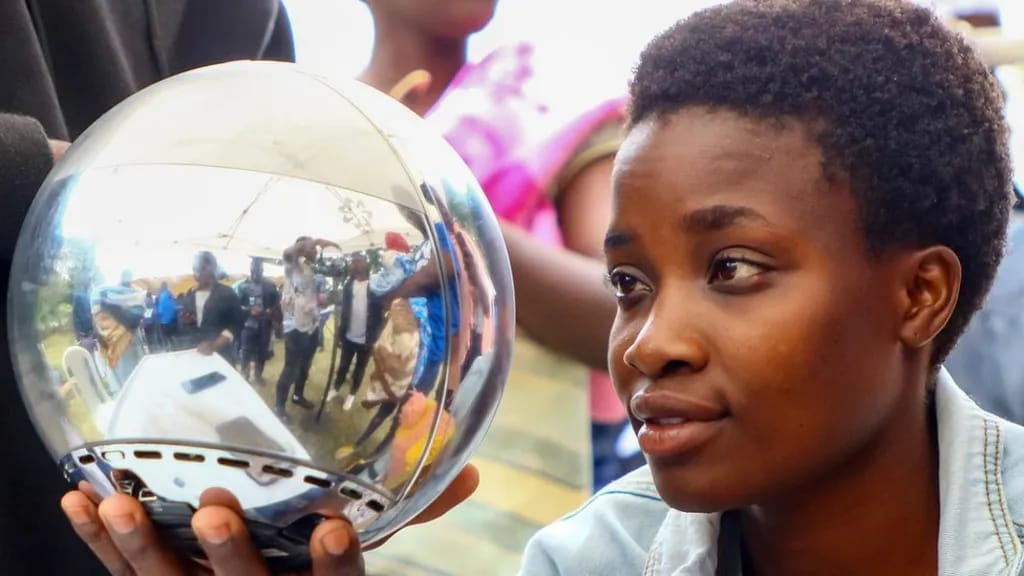
\includegraphics[width=0.5\textwidth]{kenya.jpg}
    \label{fig:kenya}
    \caption{Orbe a ler íris de uma cidadã do Kenya}
\end{wrapfigure}

Até a data de escrita deste artigo, ao adotar a Worldcoin, é concedida uma determinada quantia de moeda em sua carteira digital logo após a doação de sua íris, estabelecendo uma espécie de venda de seus dados pessoais em vez de adotar uma nova tecnologia por seus benefícios reais. Ao observar a situação mais atentamente, pode-se entender como a intenção de “prevenir fraudes” e “provar a personalidade” da empresa, na verdade, acaba desumanizando e reduzindo o usuário a um número que pode ser comprado.


\subsection{Envolvimento das autoridades}
\hspace{0.7cm}Outra condição importante a ser considerada quando se busca a segurança da sociedade é “a experiência ser aprovada por órgãos legitimados democraticamente” \cite{brey2017ethics}. No caso da Worldcoin, na Europa, ela foi autorizada pela BayLDA (Autoridade de Proteção de Dados do estado alemão da Baviera) mesmo após o ocorrido com os países africanos e asiáticos em 2022 \cite{Lomasworldcoin2023}.\par 

Esta situação levanta uma questão: Quem nos protege em relação às questões éticas? Se mesmo as organizações que deveriam regular o que é seguro para o público não conseguem ver um problema com o “criptocolonialismo” \cite{GuoWorldcoin2022}, que medidas podem ser tomadas? Até o momento da redação do artigo, as Autoridades de Proteção de Dados de Espanha e Portugal (2 dos 3 países europeus que adotaram inicialmente o Worldcoin) abriram investigações e proibiram temporariamente a recolha de dados do Worldcoin em território nacional e até exigiram a eliminação dos dados \cite{Lomasworldcoin2023}. Por que as autoridades iniciaram investigações? Iniciou-se a partir das reclamações e relatos dos próprios usuários.\par

Embora a Worldcoin pareça estar sob o GDPR (Regulamento Geral de Proteção de Dados da União Europeia), as investigações abertas e as proibições realmente trazem uma sensação de insegurança sobre como os dados pessoais dos usuários estão sendo realmente processados. Com esta situação, podemos ver cada vez mais os limites da privacidade diminuindo.\par

Tomando o exemplo da reação pública à Worldcoin, é fácil ver a concretização da opinião de Jasanoff sobre o assunto: “Surgem preocupações éticas em relação ao impacto do desenvolvimento tecnológico, com órgãos especializados muitas vezes influenciados por interesses privados.” \cite{ethicsinvention}, assim como: “Faltam órgãos legislativos, a experiência e a coragem para regular de forma eficaz.” \cite{ethicsinvention} e, finalmente: “A privatização da moralidade dentro dos órgãos de ética pode levar à alienação pública e à rejeição das normas” \cite{ethicsinvention}.\par

Em geral, podemos tomar as ações da Worldcoin como um exemplo de má ética nas tecnologias emergentes, nas palavras de Edward Snowden: “Não catalogue os globos oculares. Não use biometria para combate à fraude. Na verdade, não use biometria para nada. … O corpo humano não é um bilhete furado.” \cite{roth2023worldcoin}. E esperamos que tanto as autoridades como a empresa encontrem uma forma de trabalhar em conjunto para encontrar uma melhor abordagem para a recolha e gestão de dados.


\section{Conclusão}
Ao longo do artigo, usamos vários exemplos atuais de casos de boa e má ética em relação às tecnologias. Ao observarmos atentamente, é possível ver que mesmo dentro de um só caso, podemos chegar a mais de uma conclusão, como por exemplo, o uso de imagens por parte das AI, provando que este tipo de discussão é necessária para atender às necessidades do maior número de pessoas possível.\par
Além disso, ao garantir que os dados estejam igualmente acessíveis, sem qualquer tendenciosidade quanto à classe social ou nação, tornamos o poder da informação mais justo e ético aos olhos de todos.\par
Finalmente, para as tecnologias em acensão, ou que ainda estão por vir, a prevenção é a melhor abordagem para evitar grandes conflitos na sociedade. No geral, ao espalhar o conhecimento de uma área não tão explorada, podemos obter melhores defesas morais, pois o nosso maior defensor contra a injustiça somos nós mesmos, a sociedade. Com o tempo, por exemplo, podemos aprimorar legislações ao nosso favor, e protegermo-nos em relação à ética tecnológica.

\bibliographystyle{plain}
\bibliography{bibliography} % Entries are in the refs.bib file

\end{document}
